\chapter{Prima comunicazione su canale rumoroso}

\section{Come possiamo garantire una comunicazione perfetta in un canale imperfetto e rumoroso?}
Nella trasmissione di informazione, come stringhe di bit, in un canale di comunicazione imperfetto, esiste una probabilità che al ricevente del messaggio \textbf{non arrivi lo stesso messaggio} inviato dal mittente.

Esempi di canali di comunicazione variano dai cavi di una linea telefonica analogica ai dischi rigidi di un moderno PC, fino alle cellule riproduttive.

\section{Canale Binario Simmetrico}
Nel modello di comunicazione conosciuto come \textbf{Canale Binario Simmetrico} viene trasmesso dal mittente una stringa di bit.

\begin{minipage}{0.60\textwidth}
	Ogni bit $x$ che verrà trasmesso al ricevente può essere corrotto con probabilità $f$ (con 0 $\leq f \leq 1$) o arrivare correttamente con probabilità $1-f$.\\ Indichiamo inoltre ogni bit ricevuto come $y$.
\end{minipage}
\begin{minipage}{0.45\textwidth}
	\begin{figure}[H]
		\centering
		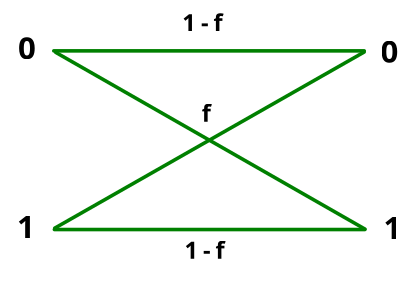
\includegraphics[width=0.5\textwidth]{images/Canale.png}
	\end{figure}
\end{minipage}

$$
P(y = 0|x= 0) = 1 -f;\quad P(y = 0| x=1) = f;
$$
$$
P(y=1|x=0) = f;\quad P(y=1|x=1) = 1 - f;
$$


\subsection{Soluzioni alla corruzione di bit in un canale di comunicazione}
Esistono in letteratura due approcci per mitigare la creazione di errori in un canale di comunicazione, la soluzione \textbf{fisica} e quella \textbf{logica}.

\textbf{Soluzione fisica}

La soluzione fisica consiste nel migliorare le caratteristiche fisiche del canale per ridurne la probabilità di errore. Tipicamente le modifiche ad un'infrastruttura fisica ne aumentano i costi.

\textbf{Soluzione sistemica}

La Teoria dell'Informazione e la Teoria dei Codici offrono un approccio diverso. Accettando di comunicare in un canale rumoroso, possiamo \textbf{trovare} e \textbf{correggere} gli errori introdotti da quest'ultimo.

Aggiungendo un \textit{encoder} prima del canale, possiamo codificare il \textbf{messaggio sorgente} $s$ nel messaggio \textbf{trasmesso} $t$, aggiungendo ad esso della \textbf{ridondanza}.\\ Il canale \textbf{corrode} il messaggio $t$ in un messaggio $r$ che, arrivato alla fine del canale, verrà decodificato da un \textit{decoder}, che userà la ridondanza per ricostruire il messaggio $s$.

\newpage
\begin{figure}[h]
	\centering
	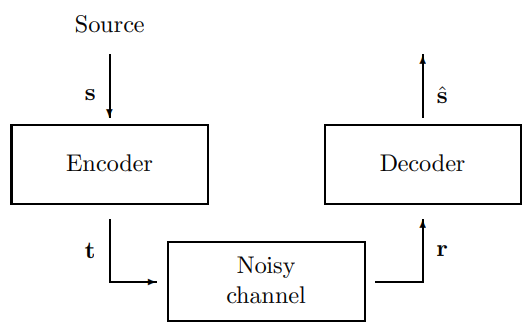
\includegraphics[width=0.5\textwidth]{images/encoder_decoder.png}
\end{figure}

Ma come possiamo aggiungere ridondanza ad un messaggio? E come possiamo \textbf{trovare} e \textbf{correggere} errori in un messaggio?

\section{Tecniche di Correzione degli errori in un Canale Binario Simmetrico}

Prima di addentrarci sulle tecniche di Error-Correction in un canale di comunicazione, è importante definire il \textbf{Tasso di Trasmissione}, ovvero:

\begin{center}
	\textit{Il rapporto tra i bit che vogliamo inviare e quelli effettivamente codificati}.
\end{center}

\subsection{Codici di Ripetizione}
Un'idea semplice per aggiungere ridondanza consiste nel \textbf{ripetere ogni bit} del messaggio $s$ per $n$ volte. Scegliendo $n$ dispari, il decoder correggerà il messaggio $r$ scegliendo il bit che compare più frequentemente in ogni sequenza di $n$ bit.

Ad esempio, se ripetessimo ogni bit 3 volte, avremmo una codifica $R_3$, quindi per ogni 3 bit sceglieremmo quello che compare almeno 2 volte.

\textbf{Esempio di Error-Correction con Codici di Ripetizione}

Immaginiamo di voler trasmettere il messaggio $s$: \verb|0110| e ipotizziamo che $f = 0.1$.\\Allora con probabilità $1-f=0.9$ il bit sarà corretto.

Utilizziamo una codifica $R_3$ per codificare il messaggio $s$ nel messaggio $t$:
$$
0 \rightarrow 000 \hspace{1cm} 1 \rightarrow 111\hspace{1cm} 1 \rightarrow 111 \hspace{1cm}0 \rightarrow 000
$$
Supponiamo che nel canale il messaggio $t$ sia stato corrotto nel messaggio $r$:
$$
010 \rightarrow 0 \hspace{1cm} 101 \rightarrow 1\hspace{1cm} 111 \rightarrow 1 \hspace{1cm}100 \rightarrow 0
$$
Nell'esempio fatto, questo semplice algoritmo ha corretto $r$ nel messaggio $s$ originale. Tuttavia i \textbf{Codici di Ripetizione} presentano due grossi limiti:
\begin{enumerate}
	\item Un Tasso di Trasmissione \textbf{molto basso}, in quanto con una codifica $R_n$, il bitrate è di soli $\frac{1}{n}$ bit.
	\item Con una cattiva distribuzione degli errori, l'algoritmo potrebbe non riuscire a correggere correttamente $r$, decodificando un $s'\neq s$. Si potrebbe aumentare la ridondanza per evitare questo scenario, ma la prima limitazione avrebbe ancora più effetto. 
\end{enumerate}

La \textbf{probabilità} di ottenere una decodifica $s'\neq s$ in una codifica $R_3$ diventa: 
$$P[E_3] = \sum^{3}_{i=2} \binom{3}{i} f^i(1-f)^{3-i}=\binom{3}{2}f^2(1-f)+f^3 = 3f^2-2f^3=O(f^2)$$
con $0\leq f \leq1$, quindi $f^2 > f^3$.

Se volessimo ridurre la probabilità di ottenere una decodifica $s'\neq s$ potremmo passare ad una codifica $R_5$. Notiamo che questa funzione vale per questo specifico canale \textbf{senza perdita} di bit.

\newpage
In $R_5$ abbiamo un tasso di pardita:
$$
P[E_5]=\sum^{5}_{i=3} \binom{5}{i}f^i(1-f)^{5-i} = \binom{5}{3} f^3(1-f)^2 + \binom{5}{4} f^4(1-f) + f^5
$$
$$
P[E_5]= 10f^3 (1-f)^2 + 5f^4(1-f) + f^5 = O(f^3)
$$

Se volessimo fare lo stesso calcolo per una decodifica $R_N$ avremmo:
$$
P[E_N]=\sum^{N}_{i=\frac{N+1}{2}} \binom{N}{i}f^i(1-f)^{N-i} = O(f^{\frac{N+1}{2}})
$$
Notiamo che la \textbf{crescita è lineare} e che dovremmo usare troppo spazio per tassi d'errore tendenti allo zero.

\textbf{Variazione con doppia codifica}

Supponiamo di codificare la stessa stringa $s$ nella codifica $R_9$. Calcolando la probabilità di ottenere una decodifica $s\neq s'$ otterremmo $P[E_9]=O(f^6)$.

Sfruttando una variante dei Codici di Ripetizione con una doppia codifica, codificando $R_9$ come $R^2_3$, cioè codificando due volte in $R_3$.\\ 
Come esempio prendiamo il messaggio $s$: \verb|1101| che con questa codifica diventa:
$$
1 \rightarrow 111 \qquad 1 \rightarrow 111 \qquad 0 \rightarrow 000 \qquad 1 \rightarrow 111 \qquad
$$
e successivamente:
$$
111 \rightarrow 111111111 \qquad 111 \rightarrow 111111111 \qquad 000 \rightarrow 000000000 \qquad 111 \rightarrow 111111111 \qquad
$$

Otteniamo: 
$$
P[E_{R^2_3}]=\sum^{3}_{i=2}\binom{3}{i}P^i_{2R_3}(1-P_{2R_3})^{3-i} \approx O(f^4)
$$
che risulta \textbf{peggiore} dell'algoritmo classico, quindi paghiamo lo spazio con l'errore.


\subsection{Codici a Blocco - Hamming (7,4)}
Possiamo ottenere trasmettere messaggi $s$ con una bassa probabilità di errore e con un tasso di trasmissione accettabile? Si, tramite i codici a \textbf{Blocchi}.

Un codice a blocco è una \textbf{regola} per convertire una sequenza di bit sorgente $s$ di lunghezza $K$ in una sequenza $t$ di lunghezza $N$, con $N > K$. Gli extra bit $N-K$ sono funzioni lineari degli originali $K$ bit e sono chiamati \textbf{bit di parità}.

Un esempio di codice a blocco lineare è il Codice di Hamming (7,4) che trasmette $N=7$ bit per ogni $K=4$ bit sorgente.
I quattro bit di informazione che vogliamo trasmettere sono indicati come $s_1, s_2, s_3, s_4$ mentre i bit di parità sono indicati con $t_1, t_2, t_3$, scelti affinché:

\begin{minipage}{0.50\textwidth}
	\begin{center}
		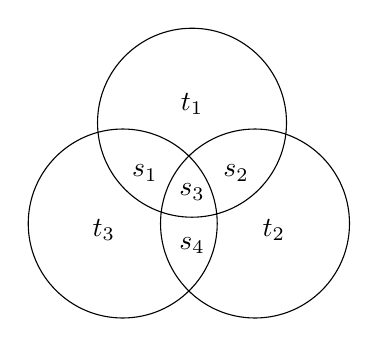
\begin{tikzpicture}[scale=0.4]
			\tikzstyle{every node}+=[inner sep=0pt]
			\draw [black] (35.7,-21.3) circle (3);
			\draw (35.1,-21.5) node {$t_3$};
			\draw [black] (37.9,-18.1) circle (3);
			\draw (37.9,-17.5) node {$t_1$};
			\draw [black] (39.9,-21.3) circle (3);
			\draw (40.5,-21.5) node {$t_2$};
			\draw (39.3,-19.7) node {$s_2$};
			\draw (36.4,-19.7) node {$s_1$};
			\draw (37.9,-22) node {$s_4$};
			\draw (37.9,-20.3) node {$s_3$};
		\end{tikzpicture}
	\end{center}
\end{minipage}
\begin{minipage}{0.45\textwidth}
	$$s_1+s_2+s_3+t_1=0 \mod2$$
	$$s_2+s_3+s_4+t_2=0 \mod2$$
	$$s_1+s_3+s_4+t_3=0 \mod2$$
\end{minipage}

Il tasso di trasmissione è $\frac{4}{7}$, \textbf{migliore} rispetto a quello dei Codici di Ripezione.
\newpage
\subsubsection{Esempio di Error-Correction con Hamming (7,4)}

Trasmettiamo nuovamente il messaggio $s$: \verb|1101|. Calcolando i bit di parità, otteniamo:

\begin{minipage}{0.50\textwidth}
	\begin{center}
		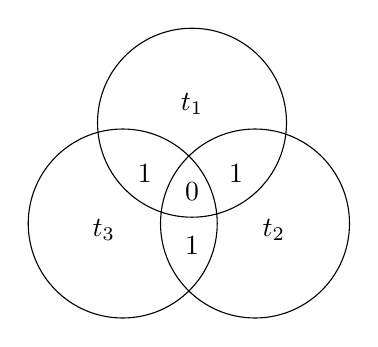
\begin{tikzpicture}[scale=0.4]
			\tikzstyle{every node}+=[inner sep=0pt]
			\draw [black] (35.7,-21.3) circle (3);
			\draw (35.1,-21.5) node {$t_3$};
			\draw [black] (37.9,-18.1) circle (3);
			\draw (37.9,-17.5) node {$t_1$};
			\draw [black] (39.9,-21.3) circle (3);
			\draw (40.5,-21.5) node {$t_2$};
			\draw (39.3,-19.7) node {$1$};
			\draw (36.4,-19.7) node {$1$};
			\draw (37.9,-22) node {$1$};
			\draw (37.9,-20.3) node {$0$};
		\end{tikzpicture}
	\end{center}
\end{minipage}
$\Rightarrow$
\begin{minipage}{0.50\textwidth}
	\begin{center}
		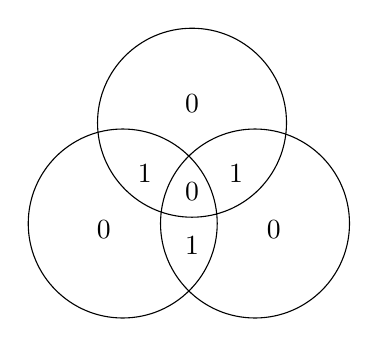
\begin{tikzpicture}[scale=0.4]
			\tikzstyle{every node}+=[inner sep=0pt]
			\draw [black] (35.7,-21.3) circle (3);
			\draw (35.1,-21.5) node {$0$};
			\draw [black] (37.9,-18.1) circle (3);
			\draw (37.9,-17.5) node {$0$};
			\draw [black] (39.9,-21.3) circle (3);
			\draw (40.5,-21.5) node {$0$};
			\draw (39.3,-19.7) node {$1$};
			\draw (36.4,-19.7) node {$1$};
			\draw (37.9,-22) node {$1$};
			\draw (37.9,-20.3) node {$0$};
		\end{tikzpicture}
	\end{center}	
\end{minipage}

Supponiamo che adesso il secondo bit del messaggio $t$ venga corrotto durante la trasmissione nel canale e che diventi il messaggio $r$: \verb|1001000|. Una volta che arriva al decoder, quest'ultimo è in grado di \textbf{individuare e correggere l'errore}, in quanto rileva una somma dispari.

\begin{minipage}{0.50\textwidth}
	\begin{center}
		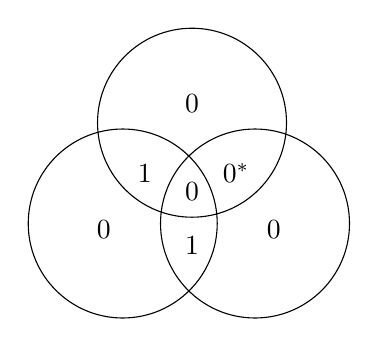
\begin{tikzpicture}[scale=0.4]
			\tikzstyle{every node}+=[inner sep=0pt]
			\draw [black] (35.7,-21.3) circle (3);
			\draw (35.1,-21.5) node {$0$};
			\draw [black] (37.9,-18.1) circle (3);
			\draw (37.9,-17.5) node {$0$};
			\draw [black] (39.9,-21.3) circle (3);
			\draw (40.5,-21.5) node {$0$};
			\draw (39.3,-19.7) node {$0^*$};
			\draw (36.4,-19.7) node {$1$};
			\draw (37.9,-22) node {$1$};
			\draw (37.9,-20.3) node {$0$};
		\end{tikzpicture}
	\end{center}	
\end{minipage}
$\Rightarrow$
\begin{minipage}{0.50\textwidth}
	\begin{center}
		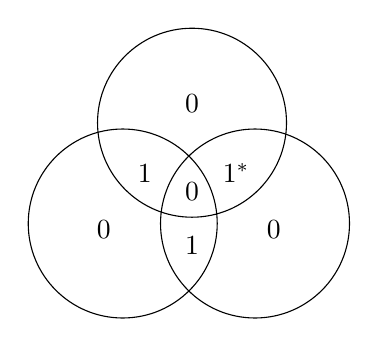
\begin{tikzpicture}[scale=0.4]
			\tikzstyle{every node}+=[inner sep=0pt]
			\draw [black] (35.7,-21.3) circle (3);
			\draw (35.1,-21.5) node {$0$};
			\draw [black] (37.9,-18.1) circle (3);
			\draw (37.9,-17.5) node {$0$};
			\draw [black] (39.9,-21.3) circle (3);
			\draw (40.5,-21.5) node {$0$};
			\draw (39.3,-19.7) node {$1^*$};
			\draw (36.4,-19.7) node {$1$};
			\draw (37.9,-22) node {$1$};
			\draw (37.9,-20.3) node {$0$};
		\end{tikzpicture}
	\end{center}	
\end{minipage}

\subsubsection{Sindrome della decodifica dei Codici di Hamming}
Supponiamo ancora una volta di voler trasmettere il messaggio $s$: \verb|1101| che viene codificato nel messaggio $t$: \verb|1101000|.
Questa volta tuttavia si corrompono i bit $s_2$ ed $s_3$ e al decoder arriva il messaggio $r$: \verb|1011000|.

\begin{center}
	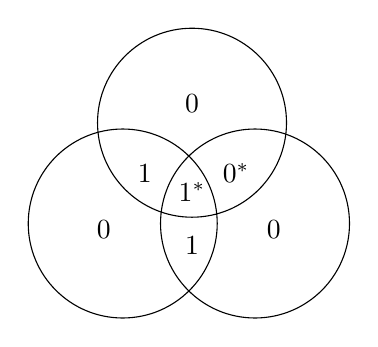
\begin{tikzpicture}[scale=0.4]
		\tikzstyle{every node}+=[inner sep=0pt]
		\draw [black] (35.7,-21.3) circle (3);
		\draw (35.1,-21.5) node {$0$};
		\draw [black] (37.9,-18.1) circle (3);
		\draw (37.9,-17.5) node {$0$};
		\draw [black] (39.9,-21.3) circle (3);
		\draw (40.5,-21.5) node {$0$};
		\draw (39.3,-19.7) node {$0^*$};
		\draw (36.4,-19.7) node {$1$};
		\draw (37.9,-22) node {$1$};
		\draw (37.9,-20.3) node {$1^*$};
	\end{tikzpicture}
\end{center}	

Il decoder procederà al rilevamento e alla correzione degli errori. Il risultato della decodifica è il seguente messaggio $s'$: \verb|1011001|, diverso da $s$.

\begin{center}
	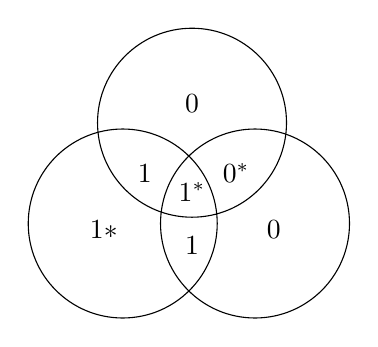
\begin{tikzpicture}[scale=0.4]
		\tikzstyle{every node}+=[inner sep=0pt]
		\draw [black] (35.7,-21.3) circle (3);
		\draw (35.1,-21.5) node {$1*$};
		\draw [black] (37.9,-18.1) circle (3);
		\draw (37.9,-17.5) node {$0$};
		\draw [black] (39.9,-21.3) circle (3);
		\draw (40.5,-21.5) node {$0$};
		\draw (39.3,-19.7) node {$0^*$};
		\draw (36.4,-19.7) node {$1$};
		\draw (37.9,-22) node {$1$};
		\draw (37.9,-20.3) node {$1^*$};
	\end{tikzpicture}
\end{center}

Ebbene, i codici di Hamming (7,4) \textbf{falliscono} nella correzione di messaggi con \textbf{almeno due errori}.\\  Sia $E_H$ l'evento che i bit vengano inviati con errori. Allora la probabilità di averne 2 è:
$$
P[E_H]=\sum^{7}_{i=2}\binom{7}{i}f^i(1-f)^{7-i}=O(f^2)
$$
uguale a quella della codifica $R_3$, ma con un tasso di trasmissione molto più elevato.

Se vogliamo un tasso d'errore alto sembrerebbe che anche il bitrate debba esserlo. Shannon ci dice che possiamo avere un tasso d'errore basso e un bitrate consistentemente diverso da 0.
